% A two-form at p eats two vectors v1, v2 and returns a real number.
% Source: book/tex/diffgeo/forms.tex (§ Multivariable forms).
\documentclass[border=2mm]{standalone}
\usepackage{tikz}\usetikzlibrary{arrows.meta}\usepackage{amssymb}
\begin{document}
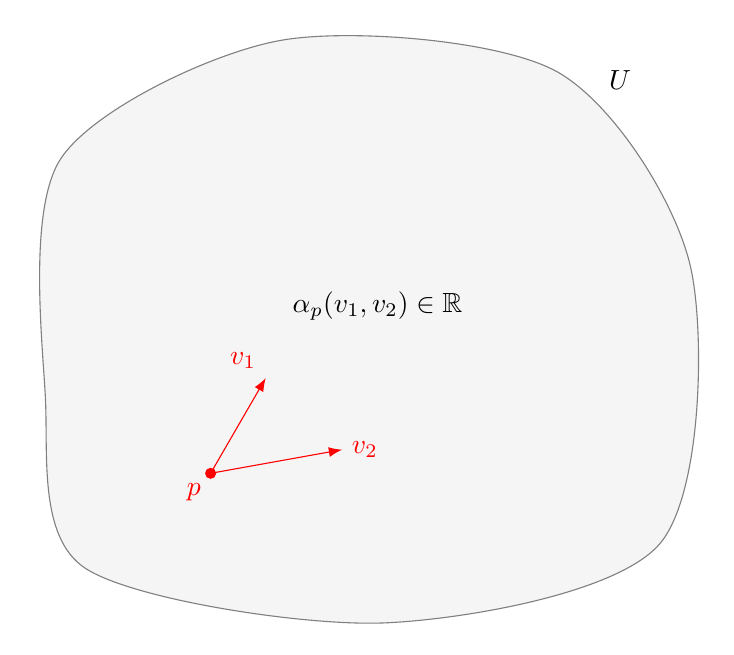
\begin{tikzpicture}
  \draw[gray,fill=gray!8] plot[smooth cycle] coordinates {(-3.6,-3.2)(0.2,-3.9)(3.7,-2.9)(4.1,0.6)(2.4,3.1)(-1.1,3.5)(-3.9,2)(-4.1,-1)}; \node at (3.2,3) {$U$};
  \fill[red] (-2,-2) circle (2pt) node[below left,red]{$p$};
  \draw[red,-{Latex}] (-2,-2)--(-1.3,-0.79) node[above left,red]{$v_1$};
  \draw[red,-{Latex}] (-2,-2)--(-0.33,-1.7) node[right,red]{$v_2$};
  \node at (0.12,0.12) {$\alpha_p(v_1,v_2)\in\mathbb{R}$};
\end{tikzpicture}
\end{document}
